\chapter{Diseño y fabricación digital} 

\label{Chapter4} 

\lhead{Capítulo 4. \emph{Diseño y fabricación}} %

%----------------------------------------------------------------------------------------
%	SECTION 1
%----------------------------------------------------------------------------------------
\begin{figure}[htbp]
	\centering
		\includegraphics[width=0.8\textwidth]{./Figures/FabDig.JPG}
	%	\rule{35em}{0.5pt}
	%\caption[Robot MODI]{robot MODI (sigla para Modular Intelligence)}
	\label{fig:MODI}
\end{figure}

Como se expuso en el capítulo anterior, actualmente existen varias alternativas de robots para comprar y construir un enjambre de robots. El problema es que o su precio es demasiado elevado o simplemente no son adaptables al tipo de investigación que se quiere realizar. Nuestro objetivo es tener un robot económico, fácil de reproducir y fabricable en la universidad para construir un enjambre de robots que permita hacer investigación y desarrollos en esta área.

\section{Diseño}

Para satisfacer los objetivos de diseño de MODI se pretende cumplir con los siguientes requerimientos:

\textbf{Requerimientos de desarrollo}

\begin{enumerate}
\item \textbf{Simple de fabricar}: Mientras más simple de fabricar sea MODI, más fácil va a ser reproducirlo para tener muchos robots en el enjambre. Esto también permite mantener los costos de fabricación bajos. 
\item \textbf{Open Source, Open Hardware}: Si se liberan tanto el código fuente del robot como la información detallada del Hardware es más fácil que otros laboratorios puedan replicar este trabajo y a su vez mejorarlo. Una de las ventajas de seguir la filosofía \textit{Open} en el desarrollo es que los que hagan uso de nuestro Hardware o Software están comprometidos a compartir sus mejoras.
\item \textbf{Fabricable en un Fab Lab}: Actualmente existen cerca de 500 Fab Labs en el mundo, así que tener un diseño compatible con las maquinarias que utilizan los Fab Labs ayuda a poder difundir este trabajo. Los componentes que no puedan ser fabricados deben ser de fácil acceso.
\item \textbf{Minimizar la cantidad de componentes mecánicos extras necesarios}: La base del diseño mecánico del robot debe ser el Chasis de éste, pieza encargada de unir todos los componentes. No debe necesitar tornillos ni silicona para ensamblarlo.
\item \textbf{Carga Autónoma}: El robot debe contar con algún sistema que facilite la carga de energía autónoma para poder realizar experimentos de larga duración sin intervención humana. Debe permitir diferentes tipos de carga como 
\item \textbf{Seguimiento de grupo}: Como se desean hacer experimentos con enjambres de robots, es necesario poder obtener la posición de cada uno de los robots.
\item \textbf{Control individual del color de cada MODI}: Para poder observar de manera rápida el estado de cada robots es necesario que cada uno cuente con un LED RGB.
\item \textbf{Movimiento simple de cada robot de forma independiente}: Cada robot debe ser capaz de recibir y ejecutar órdenes simples de movimiento en el plano.
\end{enumerate}

La función principal de MODI es ser una plataforma móvil de fácil acceso. Existe un repositorio en GitHub  \footnote{https://github.com/FabLabUChile/modi} donde se tienen los códigos actualizados para controlar y construir robots MODI. Todo esto para poder cumplir con el \textbf{requerimiento 2}. Una lista con componentes extras para comprar se encuentra en la Figura \ref{fig:BOM}. Esta lista de materiales cumple con el \textbf{requerimiento 4}.

%-----------------------------------
%	SECTION 2
%-----------------------------------

\section{Fabricación Digital}

Construir un robot implica el diseño en computador de varios componentes. Estos pueden ser circuitos electrónicos (PCB), software de control y piezas mecánicas. Uno de los requerimientos principales del desarrollo es que sea simple de fabricar, es por esto que en el resultado final se reflejan las horas de diseño.




%-----------------------------------
%	SUBSECTION 3
%-----------------------------------
\subsection{Software CAD}

CAD viene de sus siglas del Inglés, Computer-aided design, y se refiere a un diseño asistido por herramientas computacionales. Profesionales como ingenieros, arquitectos y del área del diseño por lo general son los que hacen más uso de estas herramientas.

Parte de la definición de Wikipedia es, \textit{”... se pueden dividir básicamente en programas de dibujo en dos dimensiones (2D) y modeladores en tres dimensiones (3D). Las herramientas de dibujo en 2D se basan en entidades geométricas vectoriales como puntos, líneas, arcos y polígonos, con las que se puede operar a través de una interfaz gráfica....”}

Durante el transcurso del proyecto se trabajó con varios softwares CAD. El primero fué SketchUp 8 de Google, que permite fácilmente hacer bocetos de lugares y cuenta con una importante biblioteca de modelos para incluir en el diseño. Rápidamente se pudo hacer un scketch utilizando modelos descargados de Internet , Figura~\ref{fig:setup}.




%-----------------------------------
%	SUBSECTION 2
%-----------------------------------
\subsection{Impresoras 3D}
Cuando se quiere pasar una idea al mundo real es necesario un proceso de fabricación. Dependiendo de la cantidad de herramientas que se tenga es más o menos fácil la tarea. Desde el comienzo hasta hace un par de años, quienes se dedican a construir robots, debían construir de manera \textit{artesanal} donde es imposible que las piezas queden todas iguales y el tiempo empleado era bastante. Hoy en día existe una gran alternativa, la Fabricación Digital, que surge como un nuevo paradigma de construcción y una herramienta clave para esto son las impresoras 3D. Las impresoras 3D, existen desde los 80' y hasta hace algunos años por su precio y tamaño eran de difícil acceso. Utilizan distintas tecnologías; las que se usaron en el proceso de este trabajo son las FDM, sigla del inglés "Fused deposition modeling" donde un cabezal extrusor de plástico se mueve en el plano xy depositando capa por capa de material mientras avanza en el eje z. Primero se utilizó la 3D Touch Dual de la empresa Bit from Bytes, que permite hacer modelos de hasta 185 x 273 x 200[mm], con una buena resolución de 0.125[mm]\footnote{teambastech.com/Store/index.php?route=product/product\&product\_id=205} cada capa en eje z. Luego por facilidad de uso y menor tiempo de impresión se usa una impresora MakerBot Replicator 1. También existe otro tipo de máquinas que permite hacer diseños en 2D, éstas son las cortadoras LASER. La primera versión de MODI fue construido usando planchas de madera MDF y acrílico, cortados en LASER, ver figura \ref{fig:analgTodigital} a. Hacer uso de estas máquinas permite cumplir con los \textbf{requerimientos 1 y 3}.

\begin{figure}[htbp]
	\centering
		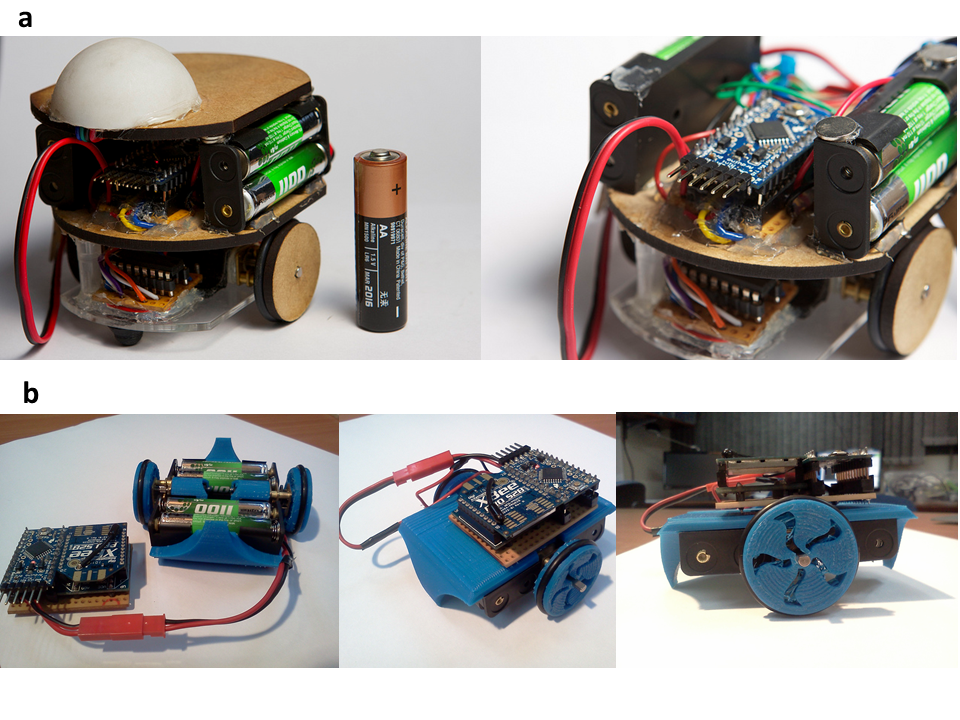
\includegraphics[width=0.8\textwidth]{./Pictures/modi_analogToDigital.png}
		\rule{35em}{0.5pt}
	\caption[Comparación de construcción análoga y digital]{\textbf{a.} Primera versión MODI construido con MDF y bastante silicona. Esta versión presentaba el problema de involucrar demasiadas partes que debían ser hechas por una persona. El microcontrolador junto con la radio inalámbrica se colocaron en una placa electrónica para prototipado. Más adelante se puede ver que fueron reemplazados por una PCB llamada Arduino FIO, que es una plataforma de desarrollo Arduino junto con un socket Xbee. Otro factor clave para descartar esta versión es que utiliza 4 pilas AAA que necesitan ser removidas para poder ser recargadas, lo que impide que en futuras versiones exista la posibilidad de una carga autónoma por parte de los Robots.\textbf{b.} MODI usando técnica de \emph{ Fabricación Digital }con chasis de plástico construido con una MakerBot Replicator 1}
	\label{fig:analgTodigital}
\end{figure}

\begin{figure}[htbp]
	\centering
		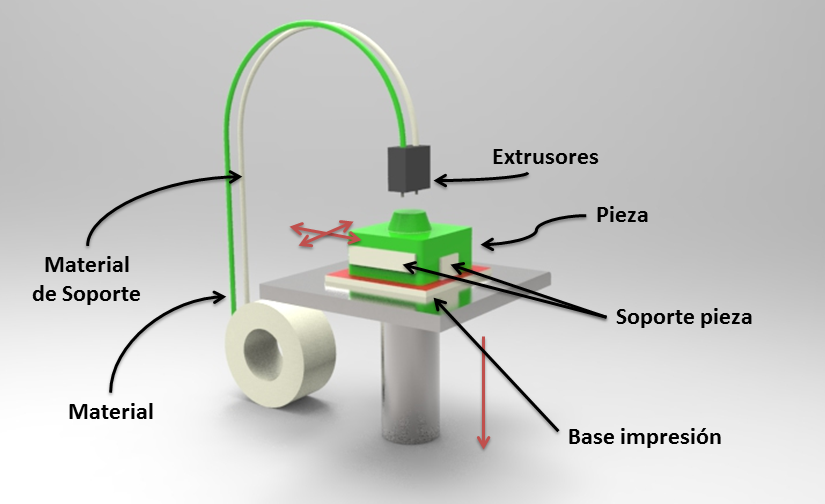
\includegraphics[width=\textwidth]{./Figures/3Dprint.png}
		\rule{35em}{0.5pt}
	\caption[Modelo funcionamiento Impresora 3D]{Modelo de funcionamiento impresoras 3D MDF. Tiene dos materiales, uno para construir la pieza y otro que funciona como soporte estructural para la impresión. Además existe una base que se calienta para sujetar la pieza mientras se construye. Puede moverse tanto la base como el extrusor para generar el modelo.}
	\label{fig:3Dprint}
\end{figure}	



\begin{figure}[htbp]
	\centering
		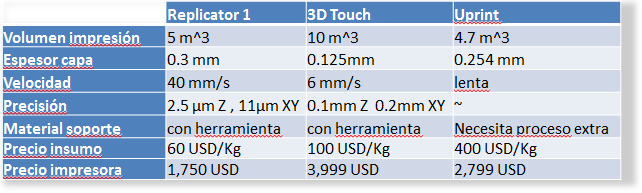
\includegraphics[width=\textwidth]{./Figures/tabla_impresoras.png}
		\rule{35em}{0.5pt}
	\caption[Tabla comparativa de impresoras 3D]{Tabla comparativa de las características más importantes de impresoras 3D, Replicator 1, 3D Touch y Uprint}
	\label{fig:TablaImpresoras}
\end{figure}


\begin{figure}[htbp]
	\centering
		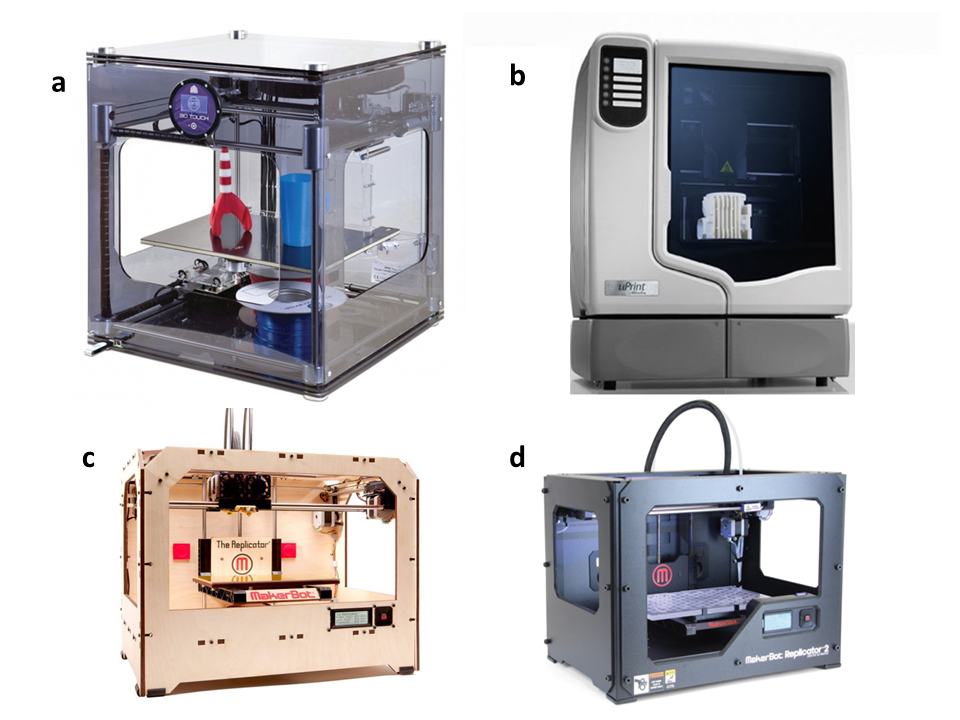
\includegraphics[width=\textwidth]{./Figures/impresoras.png}
		\rule{35em}{0.5pt}
	\caption[Impresoras 3D]{\textbf{a.} 3D Touch Dual de la empresa Bit from Bytes, \textbf{b.} Uprint SE de Stratasys, \textbf{c.} Replicator 1 de Makerbot, impresora 3D FDM utilizada para prototipar chasis y ruedas de robot MODI, \textbf{d.} Replicator 2 de MAkerbot, tiene mejor resolución que la versión 1.}
	\label{fig:impresoras}
\end{figure}	

%\FloatBarrier

Aunque han bajado los precios de las máquinas para prototipado rápido, aún no están al alcance de todas las personas. Es por esto que existen los Fab Labs (acrónimo del inglés Fabrication Laboratory), que según Wikipedia es, \textit{ "un espacio de producción de objetos físicos a escala personal o local que agrupa máquinas controladas por ordenadores. Su particularidad reside en su tamaño y en su fuerte vinculación con la sociedad."} Los Fab Labs están por todo el mundo, Figura \ref{fig:Fablabs}. MODI fue concebido como un proyecto del Fab Lab de la Universidad de Chile y por esto es posible reproducirlo en cualquier Fab Lab. En Chile, además del Fab Lab de la Universidad de Chile están: Design LAB UAI, Fab Lab Santiago y Stgo MakerSpace. 

\begin{figure}[htbp]
	\centering
		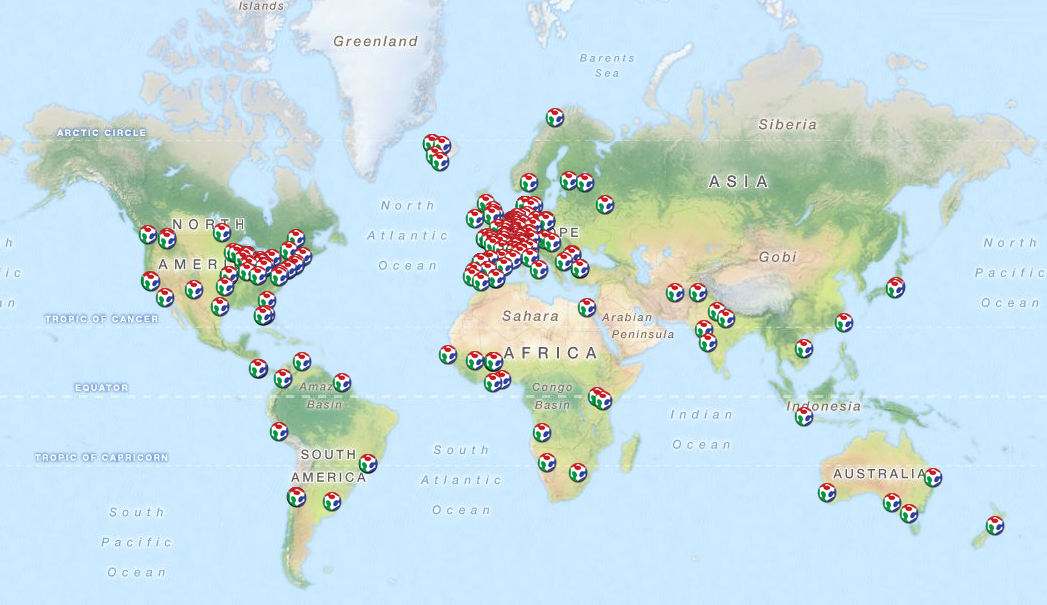
\includegraphics[width=\textwidth]{./Figures/map.png}
		\rule{35em}{0.5pt}
	\caption[Mapa Fab Labs en el mundo.]{Mapa actual de lugares en el mundo que cuentan con un Fab Lab. En Chile a la fecha existen 3. Imagen tomada de fablabamersfoort.nl/fablabs/}
	\label{fig:Fablabs}
\end{figure}	




